\section{连接杆三维建模}
\begin{procedure}
\item 切换视图方向为前视图

基于\ref{sec:lianjieganfenxi}节的连接杆建模方法分析,其中实体建模方法比较简单直接,读者可参考\ref{sec:zhoujianmo}的步骤自行完成。本节主要讲解旋转建模法构建连接杆的三维模型。从分析过程可以看出,特征面与连接杆的主视图投影方向是一致的,因此需要将视图方向切换为主视图方向。
\begin{lstlisting}
命令: -VIEW
输入选项 [?/删除(D)/正交(O)/恢复(R)/保存(S)/设置(E)/窗口(W)]: front 
\end{lstlisting}

\item 绘制特征面构成矩形

由\ref{sec:lianjieganfenxi}节的图\ref{fig:lianjieganfenxi2}可知,要构成连接轴的特征面需要绘制5个尺寸不相同的矩形。在AutoCAD中绘制矩形需要用到矩形命令,其调用方法有:
\begin{itemize}
\item 键盘输入RECTANG\index{rectang,矩形}或REC
\item 【绘图】$\rightarrow$【矩形】
\item 【绘图】$\triangleright$【矩形】图标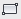
\includegraphics[scale=0.6]{rectangletool.png}
\end{itemize}

AutoCAD的矩形命令是通过矩形中的两个对角点来构造矩形的,因此需要明确两个对角点的坐标位置。
\begin{lstlisting}
命令: RECTANG
指定第一个角点或 [倒角(C)/标高(E)/圆角(F)/厚度(T)/宽度(W)]:
\end{lstlisting}

命令提示指定第一个角点时,由于此时刚开始绘图,所以只需要用鼠标在绘图区中任意点一点即可。接下来命令提示指定第二个点,根据图形我们可以看出最左边矩形的右上对角点的坐标相对于左下角点,其增量关系是$x$轴方向上增加了9mm,$y$轴方向上增加了7mm,为表达($\Delta x,\Delta y$)这种相对的坐标关系,AutoCAD采用在坐标增量前添加@符号来表示该坐标点为相对坐标。因此,我们在指定另一个角点的提示后面输入(@9,7)来表示第二个角点的坐标位置。
\begin{lstlisting}
指定另一个角点或 [面积(A)/尺寸(D)/旋转(R)]: @9,7
\end{lstlisting}

完成输入后,可以得到图\ref{fig:lianjiezhou1}所示的矩形。

\begin{figure}[htbp]
\centering
\subfloat[]{\label{fig:lianjiezhou1}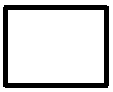
\includegraphics[scale=0.5]{lianjiezhou1.png}}\hspace{20pt}
\subfloat[]{\label{fig:endselec}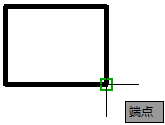
\includegraphics[scale=0.5]{endselect.png}}\hspace{20pt}
\subfloat[]{\label{fig:lianjiezho2}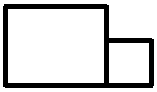
\includegraphics[scale=0.5]{lianjiezhou2.png}}
\caption{构成矩形绘制过程一}
\end{figure}

在绘制第二个矩形时,我们需要以第一矩形的右下角点做为第一点,因而输入第一点是需要将鼠标移至图\ref{fig:endselec}所示的位置,出现端点捕捉标志(绿色小矩形框),单击鼠标左键。
\begin{lstlisting}
命令: RECTANG
指定第一个角点或 [倒角(C)/标高(E)/圆角(F)/厚度(T)/宽度(W)]:
指定另一个角点或 [面积(A)/尺寸(D)/旋转(R)]: @4,4
\end{lstlisting}

完成第二个矩形的绘制后,其结果如图\ref{fig:lianjiezho2}所示。
\begin{figure}[htbp]
\centering
\subfloat[]{\label{fig:lianjiezhou3}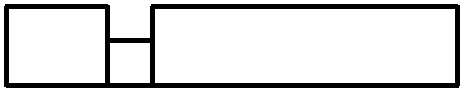
\includegraphics[scale=0.4]{lianjiezhou3.png}}\hspace{20pt}
\subfloat[]{\label{fig:lianjiezhou4}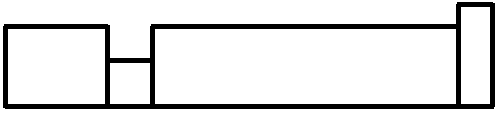
\includegraphics[scale=0.4]{lianjiezhou4.png}}
\caption{构成矩形绘制过程二}
\end{figure}

第三个矩形以第二个矩形为基础,其操作与第二矩形的操作是一致的,仅仅是对角点的坐标为(@27,7),结果如图\ref{fig:lianjiezhou3}所示。
\begin{lstlisting}
命令: RECTANG
指定第一个角点或 [倒角(C)/标高(E)/圆角(F)/厚度(T)/宽度(W)]:
指定另一个角点或 [面积(A)/尺寸(D)/旋转(R)]: @27,7
\end{lstlisting}

第四个矩形以第三个矩形为基础,其对角点坐标为(@3,9),结果如图\ref{fig:lianjiezhou4}所示。
\begin{lstlisting}
命令: RECTANG
指定第一个角点或 [倒角(C)/标高(E)/圆角(F)/厚度(T)/宽度(W)]:
指定另一个角点或 [面积(A)/尺寸(D)/旋转(R)]: @3,9
\end{lstlisting}

第五个矩形以第四个矩形为基础,其对角点坐标为(@6,7),结果如图\ref{fig:lianjiezhou5}所示。
\begin{lstlisting}
命令: RECTANG
指定第一个角点或 [倒角(C)/标高(E)/圆角(F)/厚度(T)/宽度(W)]:
指定另一个角点或 [面积(A)/尺寸(D)/旋转(R)]: @6,7
\end{lstlisting}
\item 构建面域

为了便于构建复杂的旋转特征面,需要先将绘制的矩形创建为面域。所谓面域是具有物理特性(如质心)的二维封闭线框。AutoCAD启动面域命令的方法有:
\begin{itemize}
\item 键盘输入REGION\index{region,面域}或REG
\item 【绘图】$\rightarrow$【面域】
\item 【绘图】$\triangleright$【面域】图标
\includegraphics[scale=0.6]{regiontool.png}
\end{itemize}

\begin{figure}[htbp]
\centering
\begin{floatrow}[2]
\ffigbox{\caption{构成矩形绘制结果}\label{fig:lianjiezhou5}}{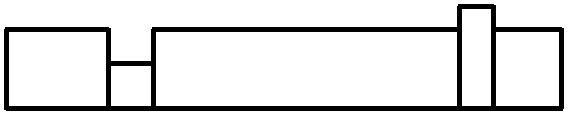
\includegraphics[scale=0.4]{lianjiezhou5.png}}
\ffigbox{\caption{面域选择结果}\label{fig:lianjiezhou6}}{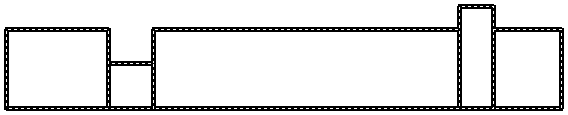
\includegraphics[scale=0.4]{lianjiezhou6.png}}
\end{floatrow}
\end{figure}

面域命令提示选择对象时,用鼠标框选绘制的5个矩形,选择后所有的矩形会以虚线形式显示,结果如图\ref{fig:lianjiezhou6}所示。
\begin{lstlisting}
命令: region
选择对象: 指定对角点: 找到 5 个
\end{lstlisting}

结束选择后,命令会提示面域操作的结果。若结果为0,通常表示面域失败经。引起失败的主要原因是选择的线框是非封闭的,或者是重复进行操作。实际中,线框不封闭是导致面域失败的主要原因。
\begin{lstlisting}
选择对象:
已提取 5 个环。
已创建 5 个面域。
\end{lstlisting}
\item 组合构成特征平面

经过面域操作后就可以用并集命令构建比较复杂的特征平面。主要是因为并集操作只能够作用于具有物理特性的面域或实体之上。组合之后的结果如图\ref{fig:lianjiezhouunion}所示。
\begin{lstlisting}
命令: UNION
选择对象: 指定对角点: 找到 5 个
选择对象:
\end{lstlisting}

\begin{figure}[htbp]
\centering
\begin{floatrow}[2]
\ffigbox{\caption{合并生成的特征面}\label{fig:lianjiezhouunion}}{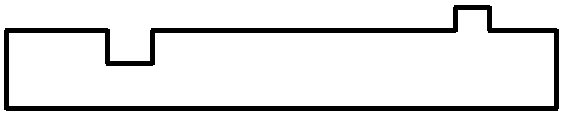
\includegraphics[scale=0.4]{lianjiezhouunion.png}}
\ffigbox{\caption{旋转操作选择结果}\label{fig:revolveselect}}{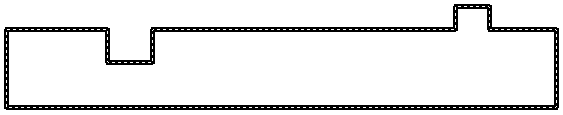
\includegraphics[scale=0.4]{revolveselect.png}}
\end{floatrow}
\end{figure}
\item 旋转生成接杆三维模型

旋转特征面构建完成后,需要AutoCAD的实体旋转命令来完成连接杆零件的三维模型构建,启动实体旋转命令的方法有:
\begin{itemize}
\item 键盘输入revolve\index{revolve,实体旋转}或rev。
\item 【绘图】$\rightarrow$【旋转】
\item 【建模】$\triangleright$【旋转】图标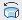
\includegraphics[scale=0.6]{solidrevolve.png}。
\end{itemize}

实体旋转命令调用后,选择特征面作为旋转对象,选择后会以图\ref{fig:revolveselect}所示的虚线方式显示。
\begin{lstlisting}
命令: REVOLVE
当前线框密度:  ISOLINES=4,闭合轮廓创建模式 = 实体
选择要旋转的对象或 [模式(MO)]: 找到 1 个
选择要旋转的对象或 [模式(MO)]:
\end{lstlisting}

\begin{figure}[htbp]
\centering
\subfloat[]{\label{fig:revolvecenter1}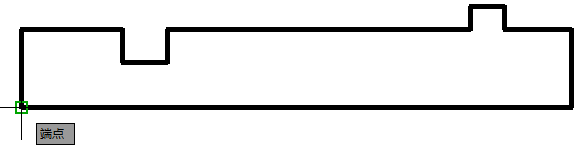
\includegraphics[scale=0.4]{revolvecenter1.png}}\hspace{20pt}
\subfloat[]{\label{fig:revolvecenter2}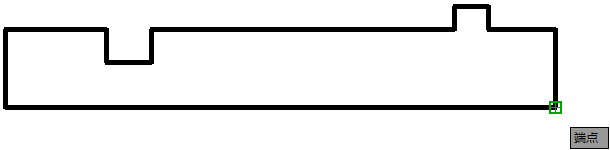
\includegraphics[scale=0.4]{revolvecenter2.png}}
\caption{定义旋转轴}
\end{figure}

选择完旋转对象后,按照图\ref{fig:revolvecenter1}所示方式,用端点捕足选择旋转轴的起点。
\begin{lstlisting}
指定轴起点或根据以下选项之一定义轴 [对象(O)/X/Y/Z] <对象>:
\end{lstlisting}

接下来,以图\ref{fig:revolvecenter2}的方式,选择轴端点。
\begin{lstlisting}
指定轴端点:
\end{lstlisting}

最后,指定旋转角度,默认为360度。
\begin{lstlisting}
指定旋转角度或 [起点角度(ST)/反转(R)/表达式(EX)] <360>:
\end{lstlisting}

旋转完成后,结果如图\ref{fig:revolveresult}所示。
\item 切换视图方向致西南等轴测

连接杆现在还剩下两个倒角尚未完成,因此先将视图方向切换为西南等轴测,以便于选择倒角边。
\begin{lstlisting}
命令: -VIEW
输入选项 [?/删除(D)/正交(O)/恢复(R)/保存(S)/设置(E)/窗口(W)]: swiso 
\end{lstlisting}

\begin{figure}[htbp]
\centering
\begin{floatrow}[2]
\ffigbox{\caption{旋转操作结果}\label{fig:revolveresult}}{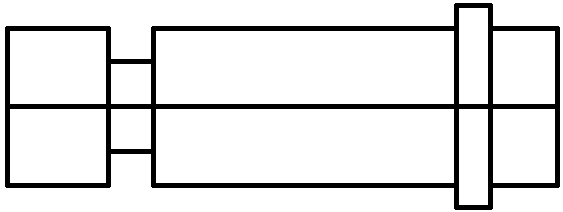
\includegraphics[scale=0.4]{revolveresult.png}}
\ffigbox{\caption{倒角结果}\label{fig:lianjieganchamferedge}}{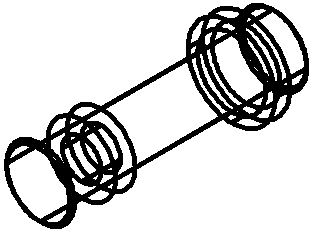
\includegraphics[scale=0.4]{lianjieganchamferedge.png}}
\end{floatrow}
\end{figure}
\item 倒角

先完成$\phi 14$长9mm圆柱体的倒角。
\begin{lstlisting}
命令: CHAMFEREDGE
距离 1 = 1.0000,距离 2 = 1.0000
选择一条边或 [环(L)/距离(D)]: d
指定距离 1 或 [表达式(E)] <1.0000>: 0.5
指定距离 2 或 [表达式(E)] <1.0000>: 0.5
选择一条边或 [环(L)/距离(D)]:
选择同一个面上的其他边或 [环(L)/距离(D)]:
按 Enter 键接受倒角或 [距离(D)]:
\end{lstlisting}

再完成$\phi 14$长6mm圆柱体的倒角。
\begin{lstlisting}
命令:  CHAMFEREDGE
距离 1 = 0.5000,距离 2 = 0.5000
选择一条边或 [环(L)/距离(D)]:
选择同一个面上的其他边或 [环(L)/距离(D)]:
按 Enter 键接受倒角或 [距离(D)]:
\end{lstlisting}
\item 切换视觉样式
\begin{lstlisting}
命令: vscurrent
输入选项 [二维线框(2)/线框(W)/隐藏(H)/真实(R)/概念(C)/着色(S)/带边缘着色(E)/灰度(G)/勾画(SK)/X 射线(X)/其他(O)] <二维线框>: g
\end{lstlisting}

最终的连接杆建模结果如图\ref{fig:lianjieganresult}所示。
\begin{figure}[htbp]
\centering
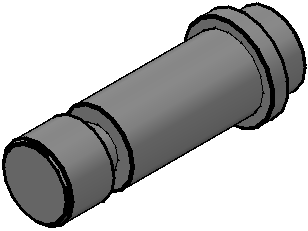
\includegraphics[scale=0.7]{lianjieganresult.png}
\caption{连接杆三维模型结果}\label{fig:lianjieganresult}
\end{figure}

\item 保存三维模型

完成后,将连接杆的三维模型以“连接杆.dwg”的文件名予以保存。
\end{procedure}
\endinput